\chapter{Data Collection} \label{chap:data}

As described in Section \ref{sec:ageDB} there are many age-based databases of facial images. However, all existing datasets are based on real age estimation. 

The idea of this work is to compare the performance between predicting real or apparent age labels. In order to do so, a web-based application has been developed using \textit{Facebook's API} to collect a database with these annotations.


\section{Web Application}

The aim of the web-based application was to speed up the collection and labelling processes and reach more people with broader backgrounds to create an age database as diverse as possible. These processes were implemented in a "gamified"\footnote{Gamification is the use of game thinking and game mechanics in non-game contexts to engage users in solving problems and increase users' self contributions. \cite{Deterding:2011:GDE:2181037.2181040}} fashion so the experience of the users with the application was satisfactory and engaging. 

The application uses the API of Facebook to create a ranking with the user's Facebook friends and add a factor of competitiveness to the game, and also to collect information about the labellers such as gender, age and nationality.

\begin{figure}[!h]
	\centering
	\begin{subfigure}[b]{0.3\textwidth}
		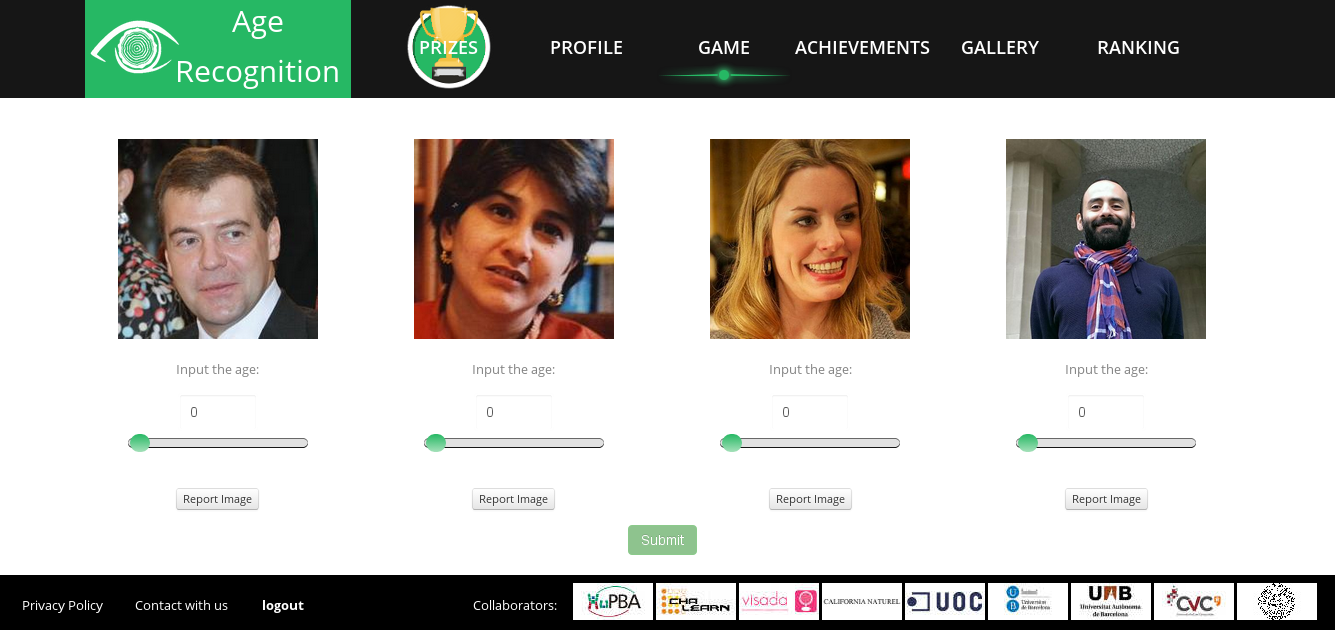
\includegraphics[width=\textwidth]{figures/age_app_1}
		\caption{Game Panel}
		\label{fig:game}
	\end{subfigure}%
	~ %add desired spacing between images, e. g. ~, \quad, \qquad, \hfill etc.
	%(or a blank line to force the subfigure onto a new line)
	\begin{subfigure}[b]{0.3\textwidth}
		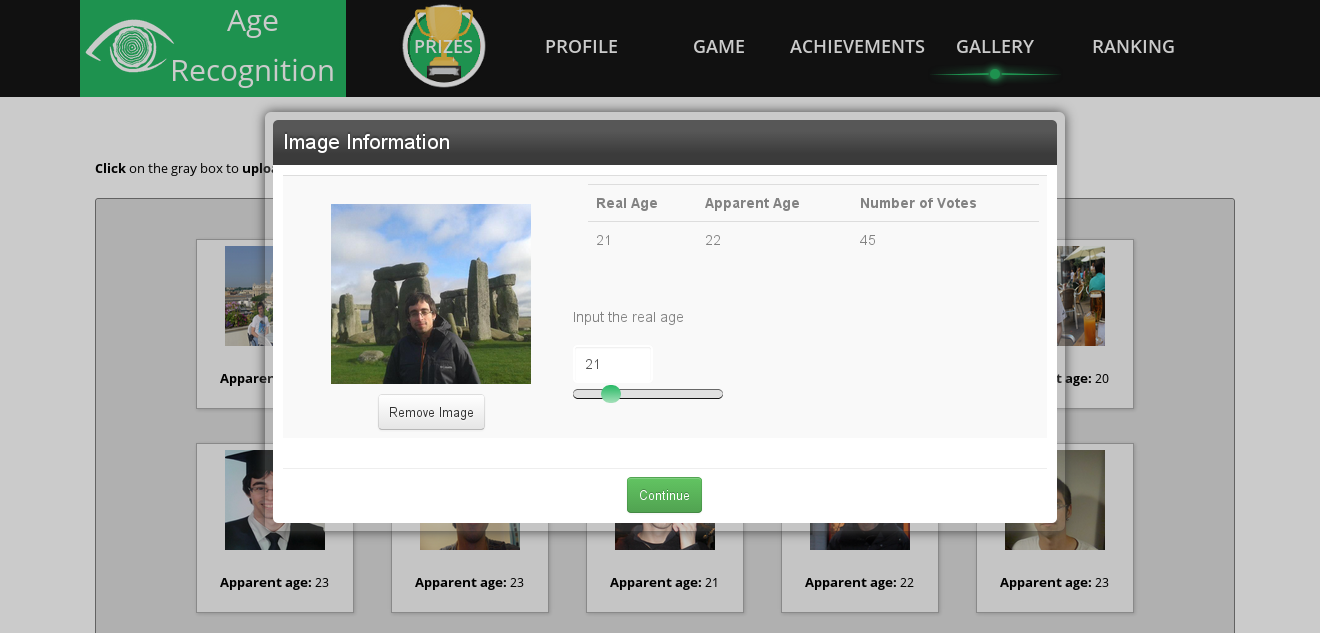
\includegraphics[width=\textwidth]{figures/age_app_2}
		\caption{Gallery Panel}
		\label{fig:gallery}
	\end{subfigure}
	~ %add desired spacing between images, e. g. ~, \quad, \qquad, \hfill etc.
	%(or a blank line to force the subfigure onto a new line)
	\begin{subfigure}[b]{0.3\textwidth}
		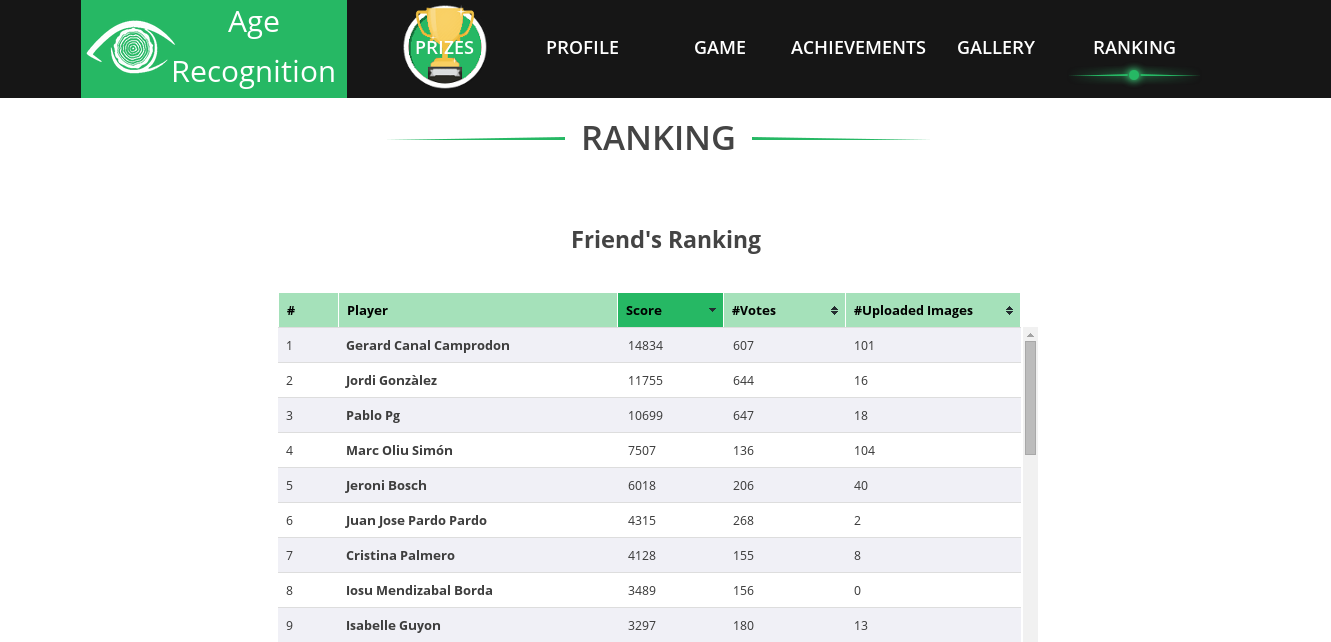
\includegraphics[width=\textwidth]{figures/age_app_3}
		\caption{Ranking Panel}
		\label{fig:ranking}
	\end{subfigure}
	\caption{Age Recognition Application. (a) User can see the images of the rest of participants and vote for the apparent age. (b) User can upload images and see their uploads in the gallery, they also can see what is the average age the other users think the people of their uploaded images look like. (c) User can see the points they achieves by uploading and voting photos and the ranking among their friends and all the participants in the application.}\label{fig:application}
\end{figure}

\subsection{Gamification strategy}
The gamification strategies were mainly three
Ranking
Feedback points
Prizes
\subsection{Application structure}

\subsection{Implementation details}

The web application was developed in a gamified way, i.e. the users or players get points for uploading and labeling images, the closer the age guess was to the apparent age (average labeled age) the more points the player obtains. In order to increase the engagement of the players we add a global and friends leaderboard where the users can see their position in the ranking. We ask the users to upload images of a single person and we give them tools to crop the image if necessary, we also ask them to give the real age (or as close as possible) of the person in uploaded image, allowing more analysis and
comparisons with real age and apparent age.

\section{HuPBA Age Dataset}

Few weeks after release the application we have alread collected near 1000 images and near 10000 votes. These numbers will continue growing in order to generate the future competition. Some of the properties of the database which is being collected with the web application are listed below:

\begin{itemize}
	\item Thousands of faces labeled by many users.
	\item Images with background.
	\item Non-controlled environments.
	\item Non-labeled faces neither landmarks, making the estima-
	tion problem even harder.
	\item One of the first datasets in the literature including
	estimated age labeled by many users to define the ground truth
	with the objective of estimating the age.
	\item The evaluation metric will be pondered by the mean and
	the variance of the labeling by the participants.
	\item The dataset also provides for each image the real age
	although not used for recognition (just for analysis purposes).
\end{itemize}

In the same way for all the labelers we have their nationality, age, and gender, which will allow analyzing demographic and other interesting studies among the correlation of labelers. In relation to the properties of existing datasets shown in Table I, ours include labels of the real age of the individuals and the apparent age given by the collected votes, both age distributions are shown in the Figure 2. The images of our database has been taken under very different conditions, which makes it more challenging for recognition purposes.
